% hw5.tex

% !TEX program = xelatex
%%%%%%%%%%%%%%%%%%%%
% see http://mirrors.concertpass.com/tex-archive/macros/latex/contrib/tufte-latex/sample-handout.pdf
% for how to use tufte-handout
\documentclass[a4paper, justified]{tufte-handout}

% hw-preamble.tex

% geometry for A4 paper
% See https://tex.stackexchange.com/a/119912/23098
\geometry{
  left=20.0mm,
  top=20.0mm,
  bottom=20.0mm,
  textwidth=130mm, % main text block
  marginparsep=5.0mm, % gutter between main text block and margin notes
  marginparwidth=50.0mm % width of margin notes
}

% for colors
\usepackage{xcolor} % usage: \color{red}{text}
% predefined colors
\newcommand{\red}[1]{\textcolor{red}{#1}} % usage: \red{text}
\newcommand{\blue}[1]{\textcolor{blue}{#1}}
\newcommand{\teal}[1]{\textcolor{teal}{#1}}

\usepackage{todonotes}

% heading
\usepackage{sectsty}
\setcounter{secnumdepth}{2}
\allsectionsfont{\centering\huge\rmfamily}

% for Chinese
\usepackage{xeCJK}
\usepackage{zhnumber}
\setCJKmainfont[BoldFont=FandolSong-Bold.otf]{FandolSong-Regular.otf}

% for fonts
\usepackage{fontspec}
\newcommand{\song}{\CJKfamily{song}}
\newcommand{\kai}{\CJKfamily{kai}}

% To fix the ``MakeTextLowerCase'' bug:
% See https://github.com/Tufte-LaTeX/tufte-latex/issues/64#issuecomment-78572017
% Set up the spacing using fontspec features
\renewcommand\allcapsspacing[1]{{\addfontfeature{LetterSpace=15}#1}}
\renewcommand\smallcapsspacing[1]{{\addfontfeature{LetterSpace=10}#1}}

% for url
\usepackage{hyperref}
\hypersetup{colorlinks = true,
  linkcolor = teal,
  urlcolor  = teal,
  citecolor = blue,
  anchorcolor = blue}

\newcommand{\me}[4]{
    \author{
      {\bfseries 姓名:}\underline{#1}\hspace{2em}
      {\bfseries 学号:}\underline{#2}\hspace{2em}\\[10pt]
      {\bfseries 评分:}\underline{#3\hspace{3em}}\hspace{2em}
      {\bfseries 评阅:}\underline{#4\hspace{3em}}
  }
}

% Please ALWAYS Keep This.
\newcommand{\noplagiarism}{
  \begin{center}
    \fbox{\begin{tabular}{@{}c@{}}
      请独立完成作业,不得抄袭。\\
      若得到他人帮助, 请致谢。\\
      若参考了其它资料,请给出引用。\\
      鼓励讨论,但需独立书写解题过程。
    \end{tabular}}
  \end{center}
}

% \newcommand{\goal}[1]{
%   \begin{center}{\fcolorbox{blue}{yellow!60}{\parbox{0.50\textwidth}{\large
%     \begin{itemize}
%       \item 体会``思维的乐趣''
%       \item 初步了解递归与数学归纳法
%       \item 初步接触算法概念与问题下界概念
%     \end{itemize}}}}
%   \end{center}
% }

% Each hw consists of four parts:
\newcommand{\beginrequired}{\hspace{5em}\section{作业 (必做部分)}}
\newcommand{\beginoptional}{\section{作业 (选做部分)}}
\newcommand{\beginot}{\section{Open Topics}}
\newcommand{\begincorrection}{\section{订正}}
\newcommand{\beginfb}{\section{反馈}}

% for math
\usepackage{amsmath, mathtools, amsfonts, amssymb}
\newcommand{\set}[1]{\{#1\}}

% define theorem-like environments
\usepackage[amsmath, thmmarks]{ntheorem}

\theoremstyle{break}
\theorempreskip{2.0\topsep}
\theorembodyfont{\song}
\theoremseparator{}
\newtheorem{problem}{题目}[subsection]
\renewcommand{\theproblem}{\arabic{problem}}
\newtheorem{ot}{Open Topics}

\theorempreskip{3.0\topsep}
\theoremheaderfont{\kai\bfseries}
\theoremseparator{:}
\theorempostwork{\bigskip\hrule}
\newtheorem*{solution}{解答}
\theorempostwork{\bigskip\hrule}
\newtheorem*{revision}{订正}

\theoremstyle{plain}
\newtheorem*{cause}{错因分析}
\newtheorem*{remark}{注}

\theoremstyle{break}
\theorempostwork{\bigskip\hrule}
\theoremsymbol{\ensuremath{\Box}}
\newtheorem*{proof}{证明}

% \newcommand{\ot}{\blue{\bf [OT]}}

% for figs
\renewcommand\figurename{图}
\renewcommand\tablename{表}

% for fig without caption: #1: width/size; #2: fig file
\newcommand{\fig}[2]{
  \begin{figure}[htbp]
    \centering
    \includegraphics[#1]{#2}
  \end{figure}
}
% for fig with caption: #1: width/size; #2: fig file; #3: caption
\newcommand{\figcap}[3]{
  \begin{figure}[htbp]
    \centering
    \includegraphics[#1]{#2}
    \caption{#3}
  \end{figure}
}
% for fig with both caption and label: #1: width/size; #2: fig file; #3: caption; #4: label
\newcommand{\figcaplbl}[4]{
  \begin{figure}[htbp]
    \centering
    \includegraphics[#1]{#2}
    \caption{#3}
    \label{#4}
  \end{figure}
}
% for margin fig without caption: #1: width/size; #2: fig file
\newcommand{\mfig}[2]{
  \begin{marginfigure}
    \centering
    \includegraphics[#1]{#2}
  \end{marginfigure}
}
% for margin fig with caption: #1: width/size; #2: fig file; #3: caption
\newcommand{\mfigcap}[3]{
  \begin{marginfigure}
    \centering
    \includegraphics[#1]{#2}
    \caption{#3}
  \end{marginfigure}
}

\usepackage{fancyvrb}

% for algorithms
\usepackage[]{algorithm}
\usepackage[]{algpseudocode} % noend
% See [Adjust the indentation whithin the algorithmicx-package when a line is broken](https://tex.stackexchange.com/a/68540/23098)
\newcommand{\algparbox}[1]{\parbox[t]{\dimexpr\linewidth-\algorithmicindent}{#1\strut}}
\newcommand{\hStatex}[0]{\vspace{5pt}}
\makeatletter
\newlength{\trianglerightwidth}
\settowidth{\trianglerightwidth}{$\triangleright$~}
\algnewcommand{\LineComment}[1]{\Statex \hskip\ALG@thistlm \(\triangleright\) #1}
\algnewcommand{\LineCommentCont}[1]{\Statex \hskip\ALG@thistlm%
  \parbox[t]{\dimexpr\linewidth-\ALG@thistlm}{\hangindent=\trianglerightwidth \hangafter=1 \strut$\triangleright$ #1\strut}}
\makeatother

% for footnote/marginnote
% see https://tex.stackexchange.com/a/133265/23098
\usepackage{tikz}
\newcommand{\circled}[1]{%
  \tikz[baseline=(char.base)]
  \node [draw, circle, inner sep = 0.5pt, font = \tiny, minimum size = 8pt] (char) {#1};
}
\renewcommand\thefootnote{\protect\circled{\arabic{footnote}}}

\newcommand{\score}[1]{{\bf [#1 分]}}

\newcommand{\rel}[1]{\xrightarrow{#1}}
\newcommand{\dstar}{\xRightarrow[]{\ast}}
\newcommand{\dplus}{\xRightarrow[]{+}}
\newcommand{\lm}{\xRightarrow[\text{lm}]{}}
\renewcommand{\rm}{\xRightarrow[\text{rm}]{}}
\newcommand{\dpluslm}{\xRightarrow[\text{lm}]{+}}
\newcommand{\dstarlm}{\xRightarrow[\text{lm}]{\ast}}
\newcommand{\dplusrm}{\xRightarrow[\text{rm}]{+}}
\newcommand{\dstarrm}{\xRightarrow[\text{rm}]{\ast}}

\newcommand{\sep}{\;\big\lvert\;}

\newcommand{\first}{\textsc{First}}
\newcommand{\follow}{\textsc{Follow}}

% see https://tex.stackexchange.com/a/109906/23098
\usepackage{empheq}
\newcommand*\widefbox[1]{\fbox{\hspace{2em}#1\hspace{2em}}} % feel free to modify this file if you understand LaTeX well
%%%%%%%%%%%%%%%%%%%%
\title{编译原理作业 (5)}
\me{魏恒峰}{hfwei@nju.edu.cn}{}{}
\date{2021年12月03日}
%%%%%%%%%%%%%%%%%%%%
\begin{document}
\maketitle
%%%%%%%%%%%%%%%%%%%%
\noplagiarism % PLEASE DON'T DELETE THIS LINE!
%%%%%%%%%%%%%%%%%%%%
\begin{abstract}
  % \mfigcap{width = 0.85\textwidth}{figs/George-Boole}{George Boole}
  % \begin{center}{\fcolorbox{blue}{yellow!60}{\parbox{0.65\textwidth}{\large
  %   \begin{itemize}
  %     \item
  %   \end{itemize}}}}
  % \end{center}
\end{abstract}
%%%%%%%%%%%%%%%%%%%%
\beginrequired
%%%%%%%%%%%%%%%

%%%%%%%%%%%%%%%
\begin{problem}[\score{20 = 4 + 8 + 4 + 4}]
  给定下述文法$G$,
  \begin{align}
    B &\to AB \\[8pt]
    B &\to b \\[8pt]
    A &\to BA \\[8pt]
    A &\to a
  \end{align}

  \begin{enumerate}[(1)]
    \item 为后面的小题计算必要的\first{}集合与\follow{}集合;
    \item 为 $G$ 构造 $LR(1)$ 自动机;

      注意: 为了尽量统一状态编号, 便于批改, 当计算\textsc{closure}时, 请按照文法编号大小顺序加入新项。
      当计算\textsc{goto}$(I, X)$时, 请按照$I$中项的出现顺序依次考虑可能的转移符号$X$。

      要求: 给出初始状态$I_{0}$的计算方法以及\textsc{goto}($I_{0}, A$)的计算方法。
    \item 为该文法设计$LR(1)$分析表; 该文法是$LR(1)$文法吗? 请说明理由。

      要求: 请说明归约的设置条件。
    \item 为该文法设计$LALR(1)$分析表; 该文法是$LALR(1)$文法吗? 请说明理由。
  \end{enumerate}
\end{problem}

\begin{solution}
\begin{enumerate}[(1)]
    \item \first{(A)} = \{a,b\}, \first{(B)} = \{a,b\}\\
    \follow{(A)} = \{a,b\}, \follow{(B)} = \{a,b,\$\}
    \item 增广文法\\
    \begin{align*}
    B' &\to B \\[8pt]
    B &\to AB \\[8pt]
    B &\to b \\[8pt]
    A &\to BA \\[8pt]
    A &\to a
  \end{align*}
  计算初始状态$I_0$:
  \begin{itemize}
      \item $I_0$=\textsc{colsure}$(\{[B'\to \cdot B,\$]\})$
      \item $[B'\to B, \$]$推导出$[B\to\cdot AB,\$]$和$[B\to\cdot b,\$]$
      \item $[B\to\cdot AB, \$]$推导出$[A\to\cdot BA,a/b]$和$[A\to\cdot a, a/b]$
      \item $[A\to\cdot BA,a/b]$推导出$[B\to\cdot AB, a/b]$和$[B\to\cdot b,a/b]$
  \end{itemize}
  得到初始状态$I_0=\{[B'\to\cdot B,\$],[B\to\cdot AB,\$/a/b],[B\to\cdot b,\$/a/b],[A\to\cdot BA,a/b],[A\to\cdot a,a/b]\}$\\\\
  计算\textsc{goto}($I_0,A$):
  \begin{itemize}
      \item 将$[B\to A\cdot B,\$/a/b]$加入新的闭包集合并计算闭包
      \item $[B\to A\cdot B,\$/a/b]$推导出$[B\to\cdot AB,\$/a/b]$和$[B\to \cdot b,\$/a/b]$
      \item $[B\to \cdot AB,\$/a/b]$推导出$[A\to\cdot BA,a/b]$和$[A\to\cdot a,a/b]$
  \end{itemize}
  得到\textsc{goto}($I_0,A$)=$\{[B\to A\cdot B,\$/a/b],[B\to\cdot AB,\$/a/b],[B\to \cdot b,\$/a/b],[A\to\cdot BA,a/b],[A\to\cdot a,a/b]\}$\\\\
  构造$LR(1)$自动机如图\ref{fig:my_label}
  \begin{figure}
      \centering
      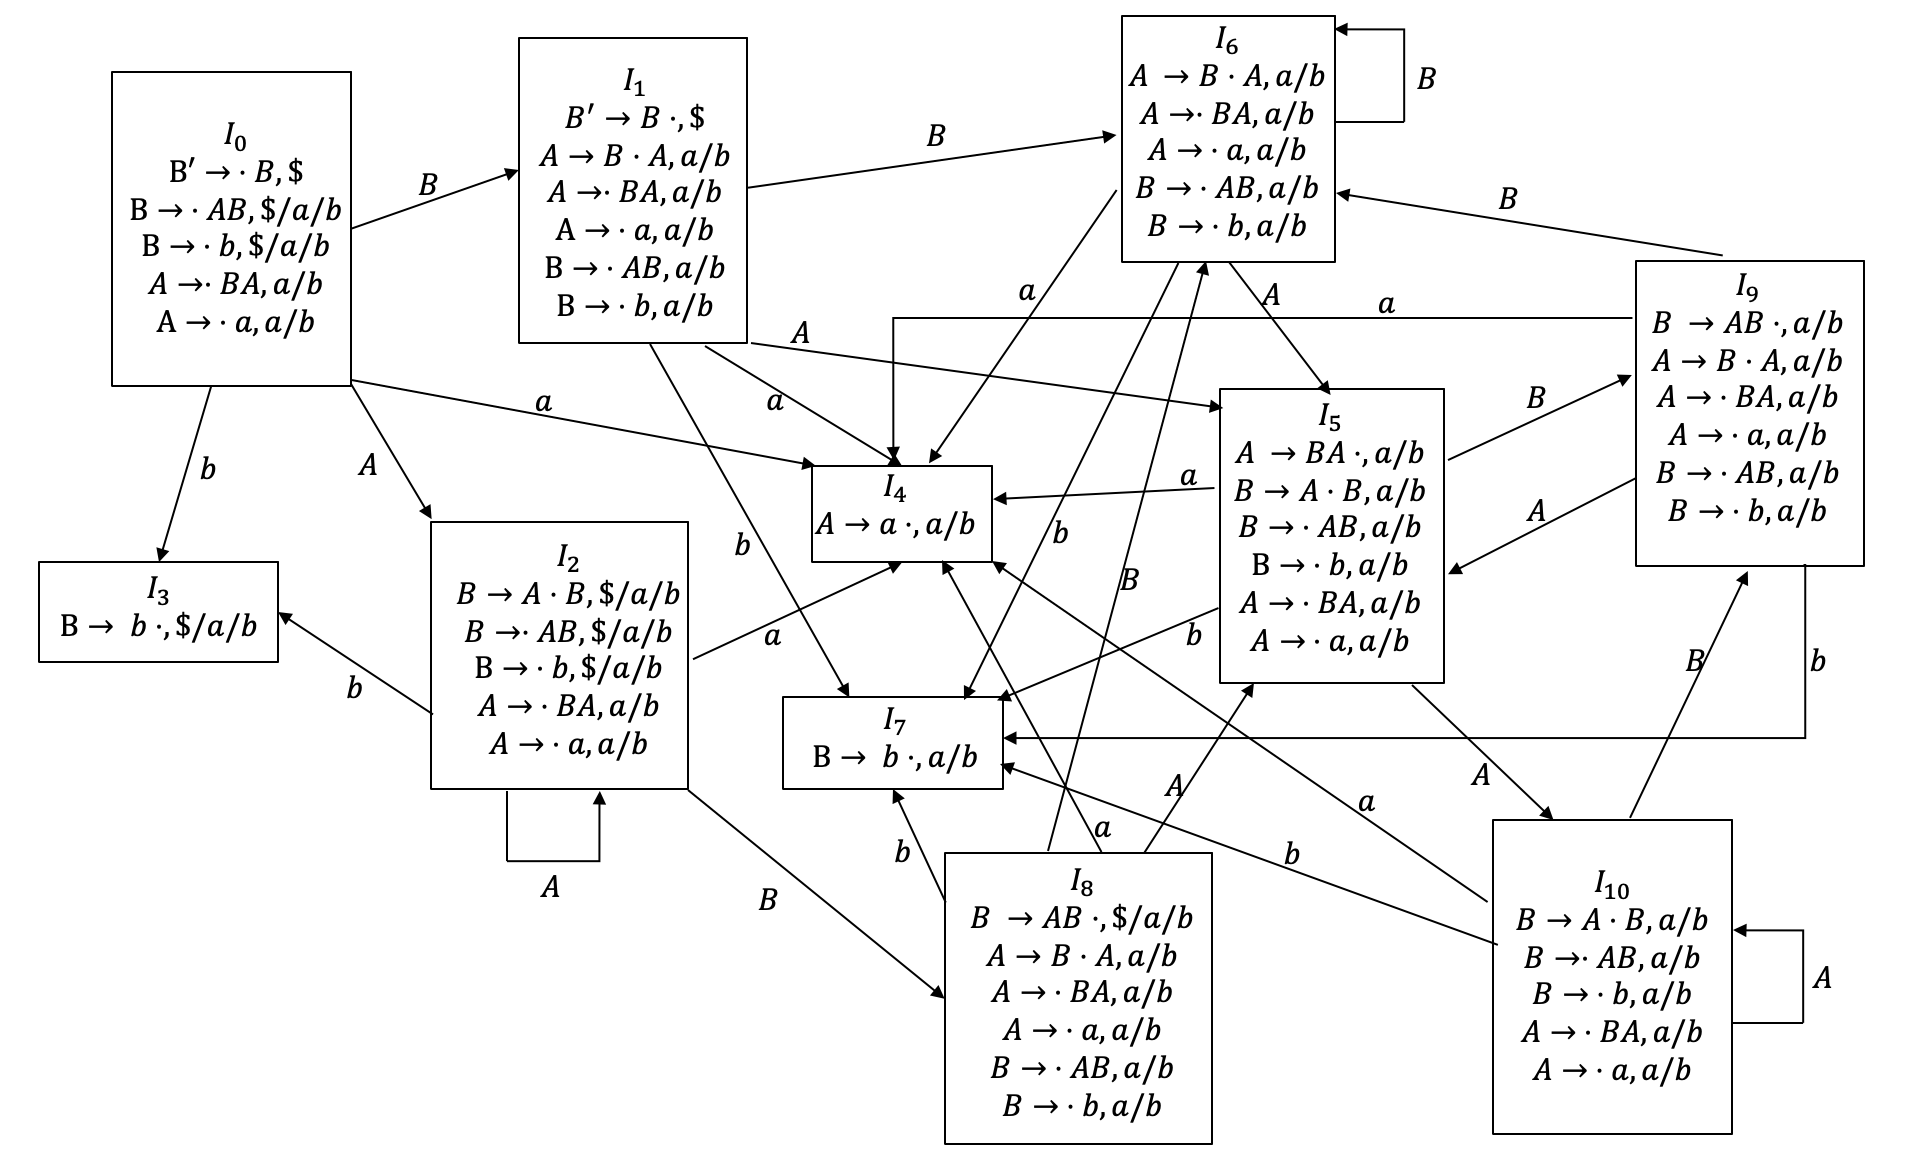
\includegraphics[scale=0.4]{fig/lr1.png}
      \caption{$LR(1)$自动机}
      \label{fig:my_label}
  \end{figure}
  \item 给出$LR(1)$分析表如表\ref{table:lr}。\\
  对于项集$I_i$,如果$[A\to \alpha, a]$在项集中,那么\textsc{ACTION}$[i,a]$按照$A\to\alpha$规约。
  不是$LR(1)$文法,因为预测分析表有冲突。
  \begin{table}[!htbp]
    \centering
    \begin{tabular}{p{2cm}|p{2cm}|p{2cm}|p{2cm}|p{2cm}|p{2cm}}
        \hline
        \hline
        \multirow{2}*{状态} & \multicolumn{3}{c|}{ACTION} & \multicolumn{2}{c}{GOTO}\\
        \cline{2-6}
        & $b$ & $a$ & $\$$ & $B$ & $A$\\
        \hline
        0 & $s3$ & $s4$ & & 1& 2\\
        1 & $s7$ & $s4$ & acc & 6 & 5\\
        2 & $s3$ & $s4$ & & 8 & 2\\
        3 & $r2$ & $r2$ & $r2$ & &  \\
        4 & $r4$ & $r4$ & & & \\
        5 & $s7/r3$ & $s4/r3$ & & 9 & 10 \\
        6 & $s7$ & $s4$ & & 6 &5 \\
        7 & $r2$ & $r2$ & & & \\
        8 & $s7/r1$ & $s4/r1$ & $r1$ & 6 & 5\\
        9 & $s7/r1$ & $s4/r1$  & & 6 & 5\\
        10 & $s7$ & $s4$ & & 9 & 10\\
        \hline
    \end{tabular}
    \label{table:lr}
  \end{table}
\item $LALR(1)$分析表如表\ref{table:lalr}。不是$LALR(1)$文法,因为预测分析表有冲突。
\begin{table}[!htbp]
    \centering
    \begin{tabular}{p{2cm}|p{2cm}|p{2cm}|p{2cm}|p{2cm}|p{2cm}}
        \hline
        \hline
        \multirow{2}*{状态} & \multicolumn{3}{c|}{ACTION} & \multicolumn{2}{c}{GOTO}\\
        \cline{2-6}
        & $b$ & $a$ & $\$$ & $B$ & $A$\\
        \hline
        0 & $s37$ & $s4$ & & 1& 2\\
        1 & $s37$ & $s4$ & acc & 6 & 5\\
        210 & $s37$ & $s4$ & & 89 & 210\\
        37 & $r2$ & $r2$ & $r2$ & &  \\
        4 & $r4$ & $r4$ & & & \\
        5 & $s37/r3$ & $s4/r3$ & & 89 & 210 \\
        6 & $s37$ & $s4$ & & 6 &5 \\
        89 & $s37/r1$ & $s4/r1$ & $r1$ & 6 & 5\\
        \hline
    \end{tabular}
    \label{table:lalr}
  \end{table}
\end{enumerate}
\end{solution}
%%%%%%%%%%%%%%%

%%%%%%%%%%%%%%%%%%%%
% 如果没有需要订正的题目,可以把这部分删掉

% \begincorrection
%%%%%%%%%%%%%%%%%%%%

%%%%%%%%%%%%%%%%%%%%
% 如果没有反馈,可以把这部分删掉
\beginfb

你可以写
\begin{itemize}
  \item 对课程及教师的建议与意见
  \item 教材中不理解的内容
  \item 希望深入了解的内容
  \item $\cdots$
\end{itemize}
%%%%%%%%%%%%%%%%%%%%
\end{document}